\documentclass{beamer}
\usecolortheme{wolverine}

% math stuff
\usepackage{amsmath}
\usepackage{amsthm}
\usepackage{amssymb}
\usepackage{xcolor}

\usepackage{float}
\usepackage{subcaption}

% to insert images
\usepackage{graphicx}

% to correctly insert stressed characters
\usepackage[T1]{fontenc}
\usepackage[utf8]{inputenc}

\usepackage{multirow}

% Bibliography
% \usepackage[style=alphabetic]{biblatex}
% \usepackage[nottoc]{tocbibind}
% \usepackage{bibentry}
% \setcounter{biburllcpenalty}{9000}
% \usepackage{nameref}

% to put links in table of contents
\usepackage{hyperref}
\hypersetup{colorlinks=false, %set true if you want colored links
    linktoc=all,     %set to all if you
}

% Add symbols
% \usepackage{textcomp}

% Add command for Real and Z sets
% \usepackage{dsfont}
% \newcommand{\Rset}{$\mathds{R}$}
% \newcommand{\Zset}{$\mathds{Z}$}

% Code highlighting
% \usepackage{minted}
% \usemintedstyle{perldoc}
% \setminted{
%     frame=single,
%     breaklines,
% }

% tikz figures
% \usepackage{tikz}
% \input{style.tikzstyle}
% \usetikzlibrary{positioning}

% number rounding
\usepackage{siunitx}
\sisetup{round-mode=places,round-precision=5}

\definecolor{myyellow}{RGB}{225, 225, 0}

\title{Thesis notes}
\date{16th March}

% any code between @(...)@ is escaped back to LaTeX
% \lstset{escapeinside={@(}{)@}}

% algorithms
\usepackage[ruled,vlined]{algorithm2e}

\begin{document}
\frame{\titlepage}

\begin{frame}[c]
    \frametitle{Negative edge fractions for many datasets}

    \begin{table}[htpb]
        \centering

        \caption{Negative edge fractions for graphs built on 200 contents of
        different subreddits}
        {\footnotesize
            \begin{tabular}{c | p{6cm} | c}
                r/cats & Pictures and videos about cats & \num{0.16922540125610608} \\
                \hline
                r/Covid19 & Scientific discussion of the pandemic & \num{0.2981398553220806} \\
                \hline
                r/programming & Computer Programming discussions & \num{0.30264993026499304} \\
                \hline
                r/climate & News about climate and related politics & \num{0.391787072243346} \\
                \hline
                r/Football & News, Rumours, Analysis about football & \num{0.41103067250904934} \\
                \hline
                r/Economics & News and discussion about economics & \num{0.41730200715730514} \\
                \hline
                r/Politics & News and discussion about U.S. politics & \num{0.5112245929821013} \\
                \hline
                r/AskTrumpSupporters & {\tiny Q\&A between Trump supporters and non
                supporters} & \num{0.5329949238578681} \\
            \end{tabular}
        }

    \end{table}

\end{frame}

\begin{frame}[c]
    \frametitle{Negative edge fraction for number of interactions}
    \begin{figure}
        \begin{center}
            \begin{subfigure}[b]{0.3\textwidth}
                \centering
                \includegraphics[width=\textwidth]{out/cats200/edge-sum-n-interactions.pdf}
                \caption{r/cats}
                % \label{fig:out/cats200/edge-sum-n-interactions.pdf}
            \end{subfigure}
            \begin{subfigure}[b]{0.3\textwidth}
                \centering
                \includegraphics[width=\textwidth]{out/programming200/edge-sum-n-interactions.pdf}
                \caption{r/programming}
                % \label{fig:out/football200/edge-sum-n-interactions.pdf}
            \end{subfigure}
            \begin{subfigure}[b]{0.4\textwidth}
                \centering
                \includegraphics[width=\textwidth]{out/asktrumpsupporters200/edge-sum-n-interactions.pdf}
                \caption{r/asktrumpsupporters}
                % \label{fig:out/football200/edge-sum-n-interactions.pdf}
            \end{subfigure}
        \end{center}
    \end{figure}

\end{frame}

\begin{frame}[c]
    \frametitle{The echo chamber problem - notation}
    \begin{itemize}
        \item $G = (V, E ^{+}, E ^{-}) $ interaction graph
        \item $ \mathcal{C} $ set of contents
        \item $C \in \mathcal{C} $ content, $\mathcal{T} _{C} $ set of threads
            associated with $C$. A thread $T \in \mathcal{T} _{C} $ is a
            subgraph of $G$
            % So $G = \bigcup _{C
            % \in \mathcal{C} } \bigcup _{T \in \mathcal{T} _C} T $ union of all
            % threads of all contents
        \item $U \subseteq V$ subset of users, $T[U]$ subgraph of $T$ induced
            by $U$. $|T(U)|$ is the number of edges of this subgraph
    \end{itemize}
\end{frame}

\begin{frame}[c]
    \frametitle{The echo chamber problem - notation}
    \begin{itemize}
        \item $\eta(C)$ fraction of negative edges associated with $C$
            (analogous definition for a thread $T$). Content (or thread)
            controversial if $\eta \in [\alpha, 1]$
        \item $\hat{\mathcal{C} } \subseteq \mathcal{C} $ set of \textit{controversial}
            contents

        \item $\mathcal{S} _C (U)$ set of \textit{non controversial} threads
            induced by $U$, for \textit{controversial} contents, i.e.

            {\small
                \begin{equation}
                    \mathcal{S} _{C} (U) = \{ T[U] \; s.t. \; T[U] \; non \;
                        controversial, T \in \mathcal{T} _{C}, C
                    \in \hat{\mathcal{C}}, U \subseteq V\}
                \end{equation}
            }
    \end{itemize}

\end{frame}

\begin{frame}[c]
    \frametitle{The echo chamber problem}
    \textbf{Goal}: given an interaction graph $G$, find $U \subseteq V$ maximing

    \begin{equation}
        \xi (U) = \sum^{}_{C \in \hat{\mathcal{C}} } \sum^{}_{T[U] \in S_C (U)}
        | T[U] |
    \end{equation}
\end{frame}

\begin{frame}[c]
    \frametitle{A possible initial implementation}

    \begin{algorithm}[H]
        \SetAlgoLined
        % \KwResult{Write here the result }
        $U = \{$ random node $\}$\;
        \While{$\xi(U)$ can be increased by adding a node}{
            With probability $\beta $  {
                add to $U$ the node increasing more the score
                $\xi(U)$ (taking into account variations in $S_C (U)$)\;
            }
            With probability $(1 - \beta )$ remove from $U$ the node increasing less the
            score $\xi(U)$. This node will be ignored in the next iteration\;
        }
        \caption{Greedy approach}
    \end{algorithm}

    \begin{itemize}
        \item Process is repeated for many nodes and maximum score is selected
        \item Final score is divided by the number of nodes of the graph.
        \item Set of users is \textit{compacted} by the random node removal
        \item $\beta $  regulates $density$ of the user group
    \end{itemize}



\end{frame}

\begin{frame}[c]
    \frametitle{About community detection}
    \begin{itemize}
        \item Follow graph may be too sparse and communities may end up
            corresponing to connected components in the interaction graph
    \end{itemize}

    \begin{figure}
        \begin{center}
            \begin{subfigure}[b]{0.4\textwidth}
                \centering
                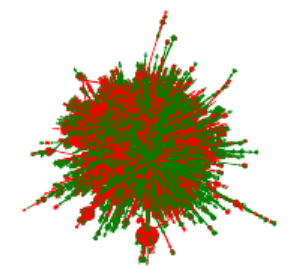
\includegraphics[width=\textwidth]{img/nytimes-giant.png}
                \caption{Giant Component, people following @nytimes}
                % \label{fig:img/nytimes-giant.png}
            \end{subfigure}
            \begin{subfigure}[b]{0.4\textwidth}
                \centering
                
\includegraphics[width=\textwidth]{img/nytimes-small1.png}
                \caption{Another component, actual group of friends discussing
                one or more contents}
                % \label{fig:}
            \end{subfigure}
        \end{center}
    \end{figure}

\end{frame}

\begin{frame}[c]
    \frametitle{An alternative to community detection: social balance}

    Distance from social balance is measured by counting \textit{frustrated}
    edges
    \footnote{\textit{From Balance and Frustration in Signed Networks} by Aref,
    Wilson}.

    Each node gets a binary label; if $x_i$ and $x_j$ labels of nodes, an edge $x _{ij} $ is frustrated if
    \begin{itemize}
        \item $x _{ij} $ is negative and $x_i = x_j$
        \item $x _{ij} $ is positive and $x_i \neq x_j$
    \end{itemize}

    The problem tries to find optimal label assignments to minimize the number of
    frustrated edges with Linear Programming.
\end{frame}

\begin{frame}[c]
    \frametitle{An alternative to community detection: social balance}
    \begin{figure}[htpb]
        \centering
        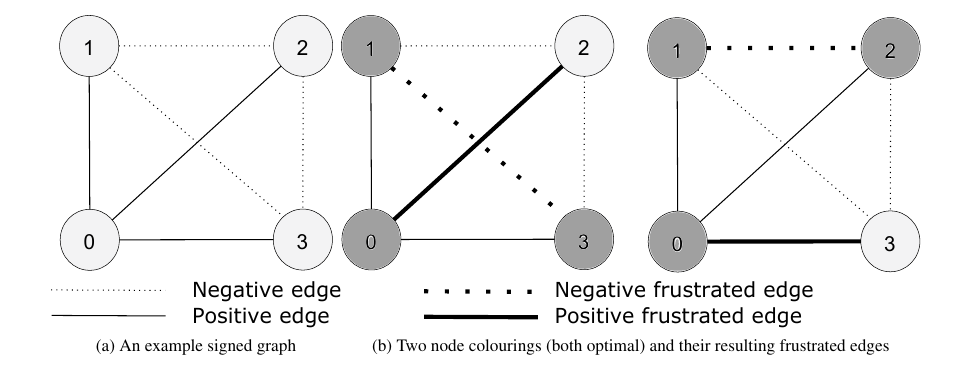
\includegraphics[width=0.8\linewidth]{img/frustration.png}
        % \caption{Name}%
        % \label{fig:name}
    \end{figure}
    \begin{itemize}
        \item Labels can be used as to identify group of users
        \item Can be called recursively to find \textit{inner} groups
    \end{itemize}
\end{frame}

\end{document}


